\documentclass[11pt]{standalone}
\usepackage{tikz, pgfplots,amsmath, amssymb, amsthm}   
\usepgfplotslibrary{groupplots}


\begin{document}

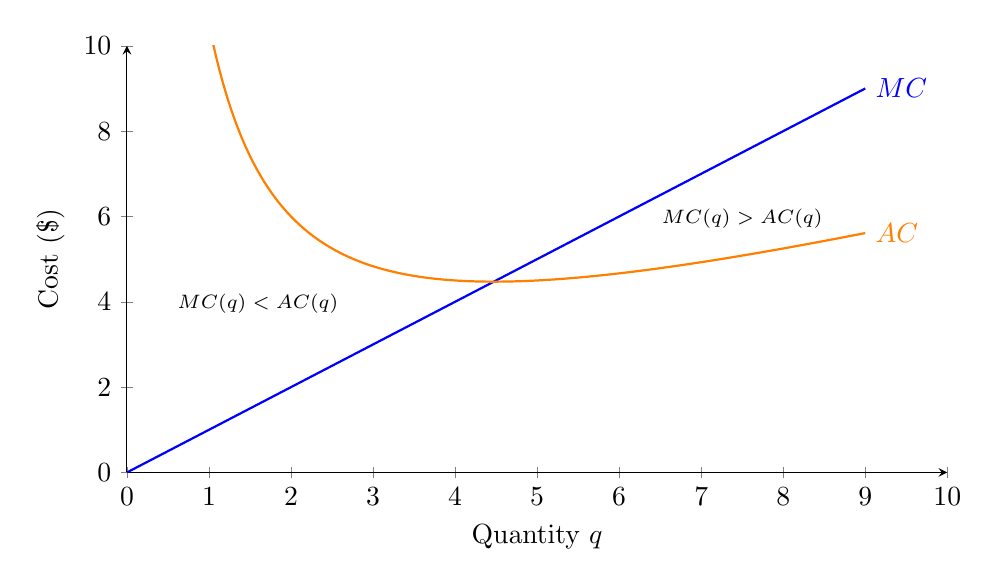
\begin{tikzpicture}
\begin{axis}[
  height=7cm, width=12cm,
  axis x line=bottom, axis y line=left,
  ylabel = Cost (\$), xlabel = Quantity $q$,
  ymin=0, ymax=10, xmin=0, xmax=10,
  extra x tick style={major tick length=0mm, grid=none},
  extra y tick style={major tick length=0mm,  grid=none},
  scatter/classes={
    a={mark=o,draw=black, mark size = 3pt},
    b={mark=*, mark size = 3pt,draw=red, fill = red}
    }
]
%\addplot[red, dashed, domain=-1:8, samples=200, variable=\t]({t},  {10+t^2/2});
  \addplot[blue, thick, domain=0:9, samples=200, variable=\t]({t},
  {t}) node[anchor= west] {$MC$} ;;
  \addplot[orange,thick, domain=0:9, samples=200, variable=\t]({t},
  {10/t+t/2}) node[anchor= west] {$AC$} ;
\addplot[scatter,only marks, scatter src=explicit symbolic]
  coordinates {
    (20, 11)     [c]
     (12, 5)      [c]
  };
\node at (axis cs:.5,3.5) [anchor=south west] {\scriptsize $MC(q)<AC(q)$};
\node at (axis cs:7.5, 5.5) [anchor=south] {\scriptsize $MC(q)>AC(q)$};
%\node at (axis cs:3, 8) [anchor=south west] {$c(q)=10+\frac{q^2}{2}$};
\end{axis}   
\end{tikzpicture}



\end{document}